%%%%%%%%%%%%%%%%%%%%%%%%%%%%%%%%%%%%%%%%%
% Beamer Presentation
% LaTeX Template
% Version 1.0 (10/11/12)
%
% This template has been downloaded from:
% http://www.LaTeXTemplates.com
%
% License:
% CC BY-NC-SA 3.0 (http://creativecommons.org/licenses/by-nc-sa/3.0/)
%
%%%%%%%%%%%%%%%%%%%%%%%%%%%%%%%%%%%%%%%%%

%----------------------------------------------------------------------------------------
%	PACKAGES AND THEMES
%----------------------------------------------------------------------------------------

\documentclass{beamer}

\mode<presentation> {

% The Beamer class comes with a number of default slide themes
% which change the colors and layouts of slides. Below this is a list
% of all the themes, uncomment each in turn to see what they look like.

%\usetheme{default}
%\usetheme{AnnArbor}
%\usetheme{Antibes}
%\usetheme{Bergen}
%\usetheme{Berkeley}
%\usetheme{Berlin}
%\usetheme{Boadilla}
%\usetheme{CambridgeUS}
%\usetheme{Copenhagen}
%\usetheme{Darmstadt}
%\usetheme{Dresden}
%\usetheme{Frankfurt}
%\usetheme{Goettingen}
%\usetheme{Hannover}
%\usetheme{Ilmenau}
%\usetheme{JuanLesPins}
%\usetheme{Luebeck}
\usetheme{Madrid}
%\usetheme{Malmoe}
%\usetheme{Marburg}
%\usetheme{Montpellier}
%\usetheme{PaloAlto}
%\usetheme{Pittsburgh}
%\usetheme{Rochester}
%\usetheme{Singapore}
%\usetheme{Szeged}
%\usetheme{Warsaw}

% As well as themes, the Beamer class has a number of color themes
% for any slide theme. Uncomment each of these in turn to see how it
% changes the colors of your current slide theme.

%\usecolortheme{albatross}
\usecolortheme{beaver}
%\usecolortheme{beetle}
%\usecolortheme{crane}
%\usecolortheme{dolphin}
%\usecolortheme{dove}
%\usecolortheme{fly}
%\usecolortheme{lily}
%\usecolortheme{orchid}
%\usecolortheme{rose}
%\usecolortheme{seagull}
%\usecolortheme{seahorse}
%\usecolortheme{whale}
%\usecolortheme{wolverine}

%\setbeamertemplate{footline} % To remove the footer line in all slides uncomment this line
%\setbeamertemplate{footline}[page number] % To replace the footer line in all slides with a simple slide count uncomment this line

%\setbeamertemplate{navigation symbols}{} % To remove the navigation symbols from the bottom of all slides uncomment this line
}
%\usepackage[usenames,dvipsnames]{color}	% Para gama de colores ver http://en.wikibooks.org/wiki/LaTeX/Colors
\usepackage{booktabs} % Allows the use of \toprule, \midrule and \bottomrule in tables
\usepackage[utf8]{inputenc}                   % Para escribir tildes y eñes
\usepackage[spanish]{babel}
\usepackage{verbatim}	% Para texto plano
\usepackage{graphicx}     % Para insertar gráficas
\DeclareGraphicsExtensions{.pdf,.png,.jpg}
\usepackage{caption}
\usepackage{amsthm}
\newtheorem{Prop}{Proposition}
%\usepackage{subcaption}


%------------------------------------------------configuración de lisnting para código de C
\usepackage{listings}	% Para códigos: C, C++, python
%\usepackage[usenames,dvipsnames,svgnames,table]{xcolor}  %http://en.wikibooks.org/wiki/LaTeX/Colors
\lstset{language=C++, basicstyle=\color{black}\ttfamily\scriptsize, keywordstyle=\color{blue}\ttfamily\scriptsize, stringstyle=\color{green}\ttfamily\scriptsize, commentstyle=\color{cyan}\ttfamily\scriptsize, morecomment=[l][\color{red}]{\#}}
%------------------------------------------------


%----------------------------------------------------------------------------------------
%	TITLE PAGE
%----------------------------------------------------------------------------------------

\title[GraphLib]{{\tiny ABSTRACT DATA STRUCTURE IN GRAPHS:}\\ Priority queue implementation for Prim's Algorithm} % The short title appears at the bottom of every slide, the full title is only on the title page

\author{Ernesto Céspedes Montero} % Your name
\institute[UCR] % Your institution as it will appear on the bottom of every slide, may be shorthand to save space
{
Universdad de Costa Rica \\ % Your institution for the title page
\medskip
\textit{netosoy@gmail.com} % Your email address
}
\date{\today} % Date, can be changed to a custom date

\begin{document}

\begin{frame}
\titlepage % Print the title page as the first slide
\end{frame}

%\begin{frame}
%\frametitle{Overview} 	% Table of contents slide, comment this block out to remove it
%\tableofcontents 		% Throughout your presentation, if you choose to use \section{} and \subsection{} commands, these will automatically be %printed on this slide as an overview of your presentation
%\end{frame}

%----------------------------------------------------------------------------------------
%	PRESENTATION SLIDES
%----------------------------------------------------------------------------------------

%------------------------------------------------
\section{Introducction} % Sections can be created in order to organize your presentation into discrete blocks, all sections and subsections are automatically printed in the table of contents as an overview of the talk
%------------------------------------------------

\begin{frame}
\frametitle{Introduction: Priority Queue}

a priority queue is an abstract data type which is like a regular queue or stack data structure, but where additionally each element has a priority''  associated with it. In a priority queue, an element with high priority is served before an element with low priority.

\begin{figure}[h]
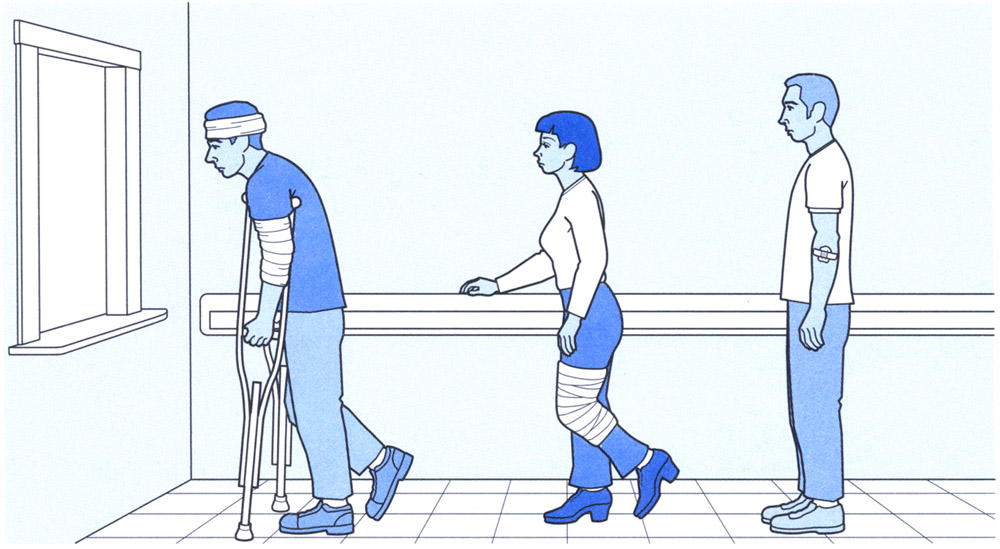
\includegraphics[width=.50\textwidth]{Images/priority.png}
\centering
\end{figure}
\end{frame}

\begin{frame}
\frametitle{Heap data struct}
\begin{itemize}
\item A heap is a tree-based data structure that satisfies the heap property: If A is a parent node of B then the key of node A is ordered with respect to the key of node B with the same ordering applying across the heap.
\end{itemize}
\begin{figure}[h]
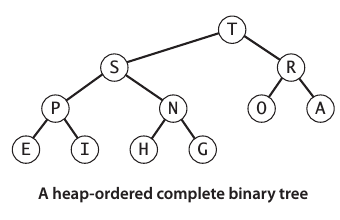
\includegraphics[width=.40\textwidth]{Images/heap1.png}
\centering
\end{figure}
\end{frame}

%------------------------------------------------

\begin{frame}
\frametitle{Heap data struct}
\begin{itemize}
\item the highest (or lowest) key is in the root node.
\item the min-heap property: the value of each node is greater than or equal to the value of its parent.
\item the max-heap property: the value of each node is less than or equal to the value of its parent.
\item heap is not a sorted structure and can be regarded as partially ordered.
\item is no particular relationship among nodes on any given level.
\end{itemize}
\begin{figure}[h]
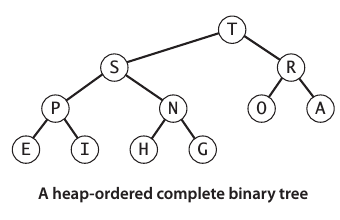
\includegraphics[width=.40\textwidth]{Images/heap1.png}
\centering
\end{figure}
\end{frame}


%------------------------------------------------
\begin{frame}
\frametitle{Heap Representation}
\begin{columns}[c] % The "c" option specifies centered vertical alignment while the "t" option is used for top vertical alignment
\column{.45\textwidth} % Left column and width
\begin{itemize}
\item the parent of the node in position $k$, is in posotion $\lfloor k/2 \rfloor$
\item the children of the node in positión $k$ are in position $2k$ and $2k+1$
\item we can travel up and down by doing simple arithmetic on array indices
\end{itemize}
\column{.5\textwidth} % Right column and width
\begin{figure}[h]
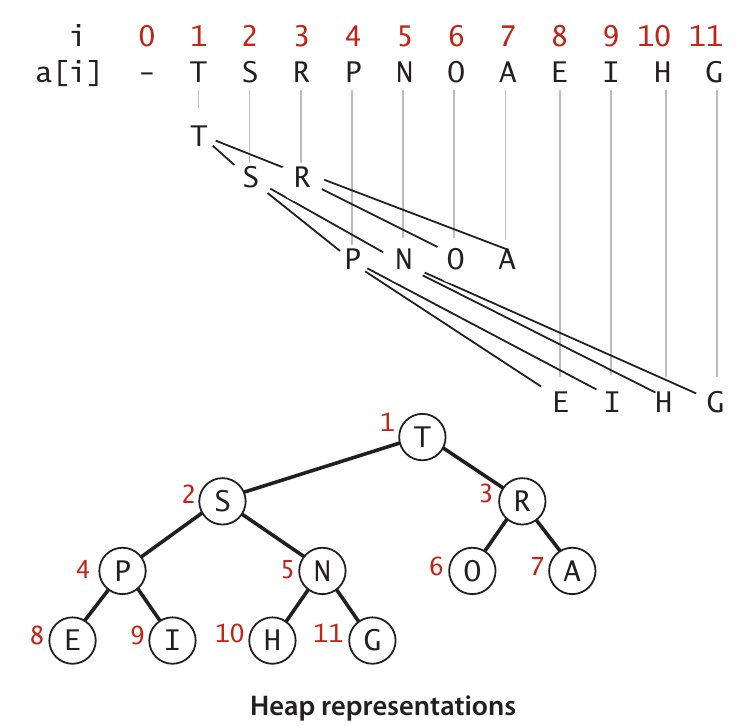
\includegraphics[width=.80\textwidth]{Images/heap2.png}
\centering
\end{figure}
\end{columns}

\end{frame}
%------------------------------------------------
\begin{frame}[fragile]
\frametitle{Max binary heap implementation}
\begin{columns}[c]
\column{.45\textwidth} % Left column and width

\begin{lstlisting}
void swap(int i, int j){
   float aux = key[i];
   key[i] = key[j];
   key[j] = aux;
   }
   
void swim(int k){	//Bottom-Up
   while(k>1 && key[k/2] < key[k]){
      swap(k/2, k);
      k = k/2;
      }
   }
\end{lstlisting}
\column{.5\textwidth} % Right column and width
\begin{figure}[h]
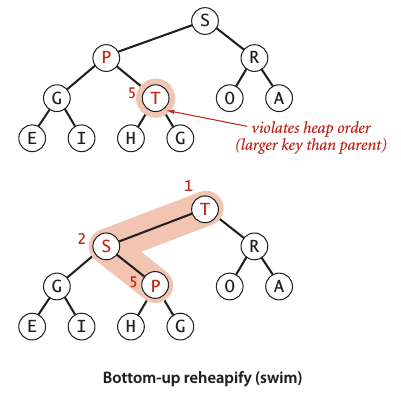
\includegraphics[width=.80\textwidth]{Images/swim.png}
\centering
\end{figure}

\end{columns}
\end{frame}
%-----------------------------------------------
\begin{frame}[fragile]
\frametitle{Max binary heap implementation}
\begin{columns}[c]
\column{.50\textwidth} % Left column and width

\begin{lstlisting}
   void sink(int k){ //Top-Down
      while(2*k <= N){
         int j = 2*k; //left child
         if(j<N && key[j] < key[j+1])
            j++;    //right child
         if(!(key[k]<key[j]))
             break;
         swap(k,j);
         k=j;
      }
   }
\end{lstlisting}
\column{.50\textwidth} % Right column and width
\begin{figure}[h]
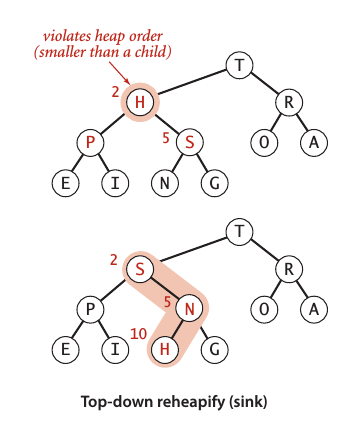
\includegraphics[width=.80\textwidth]{Images/sink.png}
\centering
\end{figure}

\end{columns}
\end{frame}
%-----------------------------------------------

\begin{frame}
\frametitle{advantages of using heaps}
\begin{itemize}
\item \textbf{Proposition} The height of a complete binary tree of size $N$ is $\lfloor log(N)\rfloor$.
\end{itemize}
\begin{figure}[h]
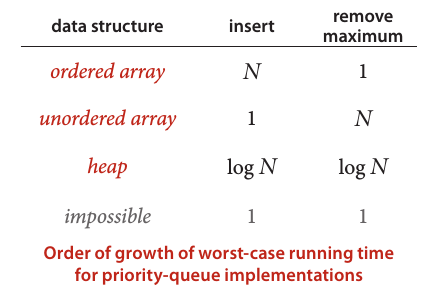
\includegraphics[width=.50\textwidth]{Images/eff.png}
\centering
\end{figure}
\end{frame}

%------------------------------------------------

\section{Heap Priority Queue} 
%-----------------------------------------------

\begin{frame}[fragile]
\frametitle{Float MaxPQ implementation}
\begin{columns}[c]
\column{.45\textwidth} % Left column and width

\begin{lstlisting}
   class MaxPQ{
   private:
      float *key;
      int N, NMAX;
   public:
      MaxPQ(int NMAX){
         this->NMAX=NMAX;
         N = 0;	
         key = new float[NMAX+1];
         }
\end{lstlisting}
\column{.5\textwidth} % Right column and width
\begin{figure}[h]
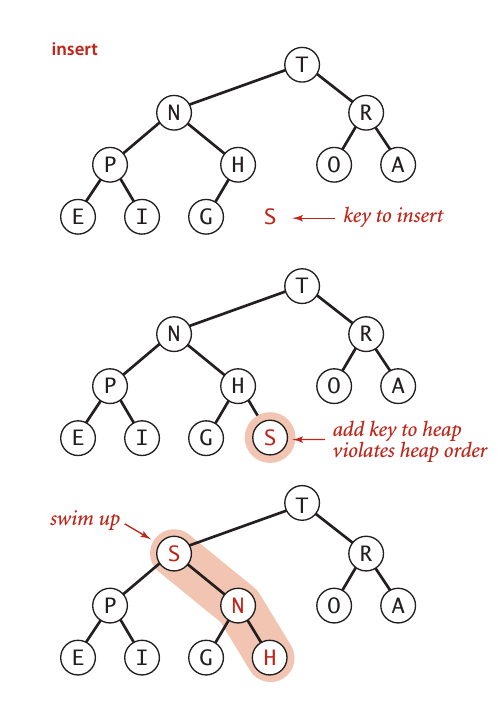
\includegraphics[width=.70\textwidth]{Images/insert.png}
\centering
\end{figure}

\end{columns}
\end{frame}

%------------------------------------------------

\begin{frame}[fragile]
\frametitle{Priority Queue: insert function}
\begin{columns}[c]
\column{.45\textwidth} % Left column and width

\begin{lstlisting}
   .
   .
   .
   
   void insert(float val){
      key[++N] = val;
      swim(N);
   }

   .
   .
   .
\end{lstlisting}
\column{.5\textwidth} % Right column and width
\begin{figure}[h]
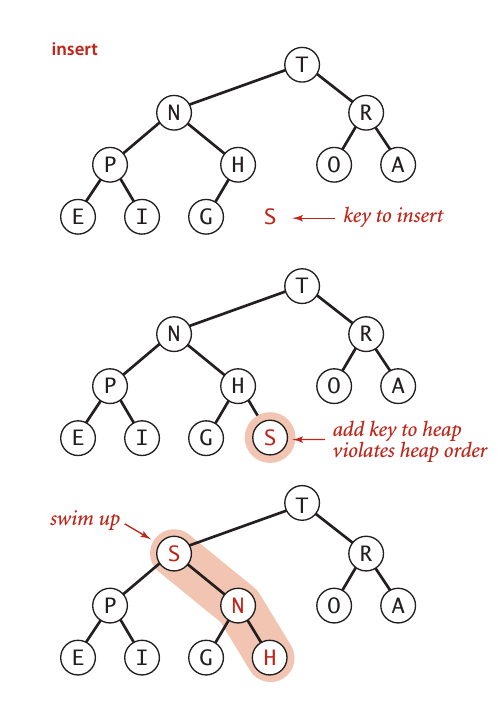
\includegraphics[width=.70\textwidth]{Images/insert.png}
\centering
\end{figure}

\end{columns}
\end{frame}
%------------------------------------------------

\begin{frame}[fragile]
\frametitle{Priority Queue: delMax function}
\begin{columns}[c]
\column{.45\textwidth} % Left column and width

\begin{lstlisting}
   .
   .
   .
   
   float delMax(void){
      float Max = key[1];
      swap(1,N--);
      key[N+1] = 0;
      sink(1);
      return Max;
   }

   .
   .
   .
\end{lstlisting}
\column{.5\textwidth} % Right column and width
\begin{figure}[h]
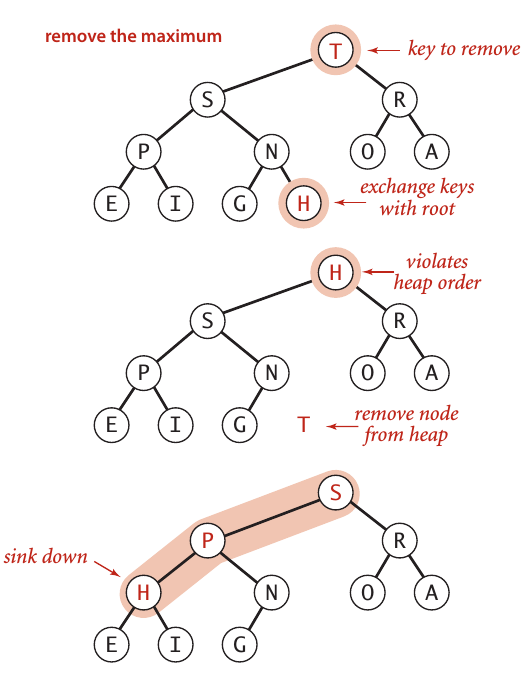
\includegraphics[width=.70\textwidth]{Images/delmax.png}
\centering
\end{figure}

\end{columns}
\end{frame}

%------------------------------------------------
%------------------------------------------------

%------------------------------------------------
\section{Application for Prim´s Algorithm}
%------------------------------------------------

\begin{frame}
\frametitle{Edge-wheigthed graph representation}
\begin{figure}[h]
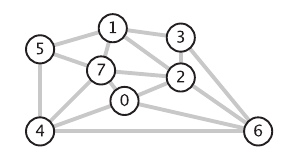
\includegraphics[width=.30\textwidth]{Images/EdgWeiGra2.png}
\centering
\end{figure}
\vspace{-5mm}
\begin{figure}[h]
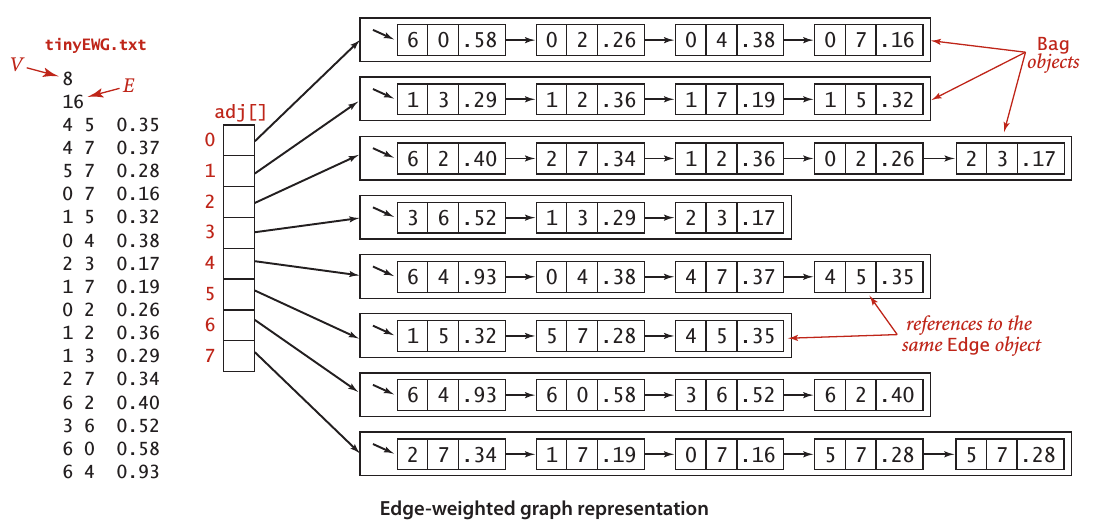
\includegraphics[width=.70\textwidth]{Images/EdgWeiGra.png}
\centering
\end{figure}
\end{frame}

%----------------------------------------------
\begin{frame}
\frametitle{Prim's Algorithm}
Prim's algorithm is based on the cut property
\begin{Prop}[Cut property]
Given any cut in an edge-weighted graph, the crossing edge of minimum weight is in the MST of the graph.
\end{Prop}
\begin{figure}[h]
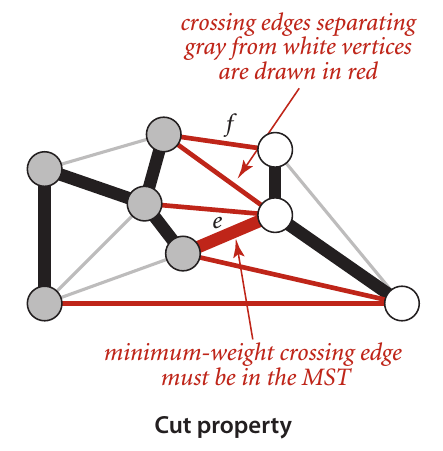
\includegraphics[width=.45\textwidth]{Images/CutProp.png}
\centering
\end{figure}
\end{frame}

%------------------------------------------------
\begin{frame}
\frametitle{Prim's Algorithm}
We implement Prim’s algorithm with the aid of simple data structures 
\begin{columns}[c] % The "c" option specifies centered vertical alignment while the "t" option is used for top vertical alignment
\column{.45\textwidth} % Left column and width
\begin{itemize}
\item {\footnotesize We use a vertex-indexed boolean array \texttt{Marked[]}, were \texttt{Marked[v]} is true if v is on the tree}
\item {\footnotesize We use a queue to collect MST edges}
\item {\footnotesize We use a MinPQ$<$Edge$>$ priority queue that compares edges by weight}
\end{itemize}
\column{.5\textwidth} % Right column and width
\begin{figure}[h]
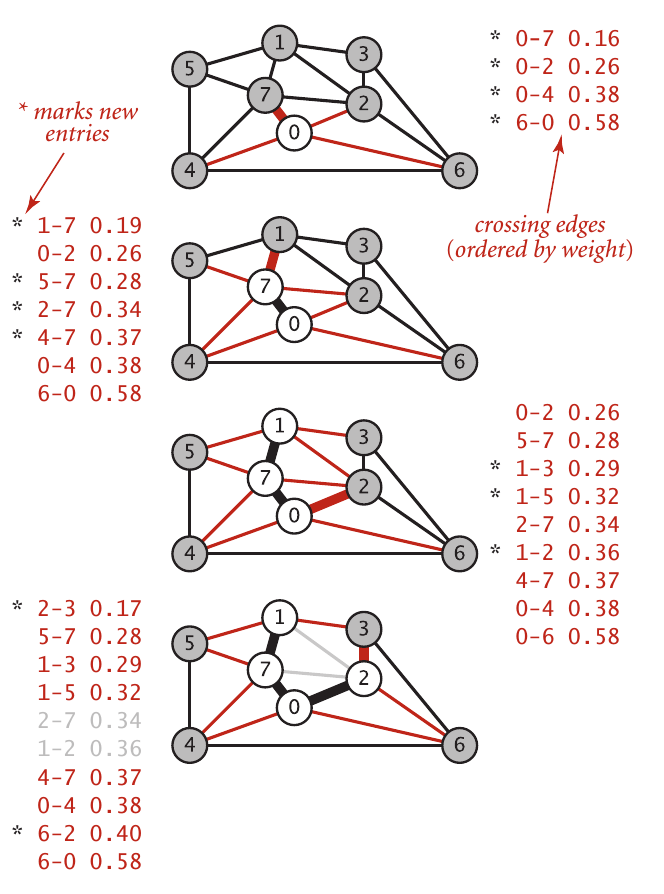
\includegraphics[width=.80\textwidth]{Images/Prim1.png}
\centering
\end{figure}
\end{columns}

\end{frame}
%----------------------------------------------
\begin{frame}
\frametitle{Prim's Algorithm}
{\footnotesize We use a private method visit() that puts a vertex on the tree, by marking it as visited and then putting all of its incident edges that are not ineligible onto the priority queue, thus ensuring that the priority queue contains the crossing edges from tree vertices to non-tree vertices.}
\begin{figure}[h]
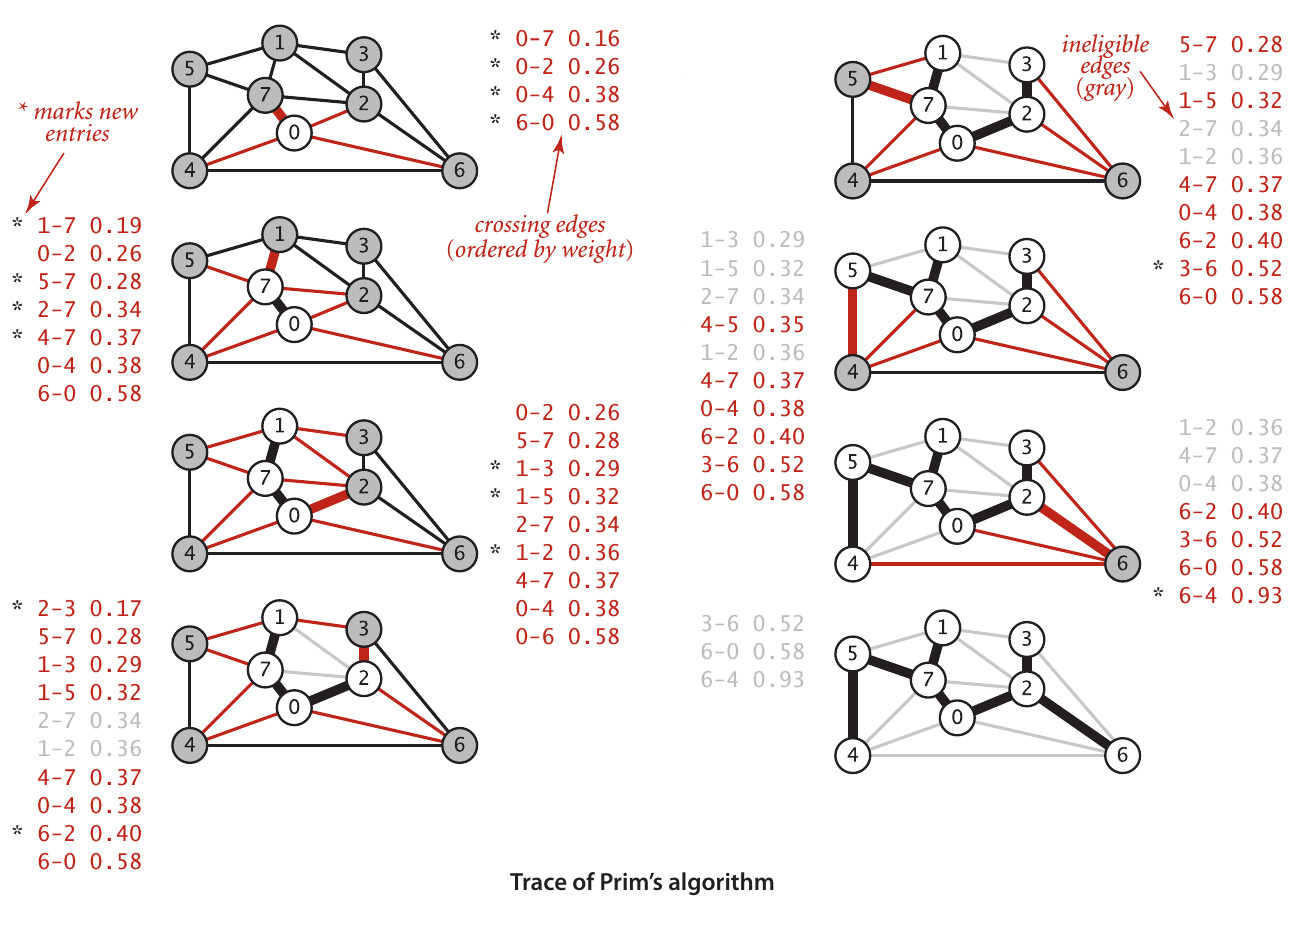
\includegraphics[width=.7\textwidth]{Images/Prim.png}
\centering
\end{figure}
\end{frame}
%----------------------------------------------------------------------------------------
\begin{frame}
\frametitle{Prim's Algorithm}
\begin{center}
{\Huge Thanks!}
\end{center}
\end{frame}

\end{document} 